% -*- TeX-engine: xetex; eval: (auto-fill-mode 0); eval: (visual-line-mode 1); -*-
% Compile with XeLaTeX

%%%%%%%%%%%%%%%%%%%%%%%
% To do before class
%%%%%%%%%%%%%%%%%%%%%%%

% Print off Readiness Assessment 1

% Send email about registering clicker.
% Test run readiness assessment on iClicker.
% I need to get scratch off sheet from Mine.

% Send the Logistics/Week0Annoucnement (the night before).
% Send an email reminding students to bring a charged computer (the night before).

% Questions for Mine
% Can I get scratch off sheets.
% What do you do during group portion?
% Question: voluntary vs. non-response

%%%%%%%%%%%%%%%%%%%%%%%
% Option 1: Slides: (comment for handouts)   %
%%%%%%%%%%%%%%%%%%%%%%%
%
%\documentclass[slidestop,compress,mathserif,12pt,t,professionalfonts,xcolor=table]{beamer}
%
%% solution stuff
%\newcommand{\solnMult}[1]{
%\only<1>{#1}
%\only<2->{\red{\textbf{#1}}}
%}
%\newcommand{\soln}[1]{\textit{#1}}

%%%%%%%%%%%%%%%%%%%%%%%%%%%%%%%
% Option 2: Handouts, without solutions (post before class)    %
%%%%%%%%%%%%%%%%%%%%%%%%%%%%%%%

 \documentclass[11pt,containsverbatim,handout,xcolor=xelatex,dvipsnames,table]{beamer}

 % handout layout
 \usepackage{pgfpages}
 \pgfpagesuselayout{4 on 1}[letterpaper,landscape,border shrink=5mm]

 % solution stuff
 \newcommand{\solnMult}[1]{#1}
 \newcommand{\soln}[1]{}

 % % This breaks things for me for some reason.
 % tell pgfpages how to set page sizes in XeLaTeX
 \renewcommand\pgfsetupphysicalpagesizes{%
    \pdfpagewidth\pgfphysicalwidth\pdfpageheight\pgfphysicalheight%
 }

%%%%%%%%%%%%%%%%%%%%%%%%%%%%%%%%%%%%
% Option 3: Handouts, with solutions (may post after class if need be)    %
%%%%%%%%%%%%%%%%%%%%%%%%%%%%%%%%%%%%

% \documentclass[11pt,containsverbatim,handout,xcolor=xelatex,dvipsnames,table]{beamer}

% % handout layout
% \usepackage{pgfpages}
% \pgfpagesuselayout{4 on 1}[letterpaper,landscape,border shrink=5mm]

% % solution stuff
% \newcommand{\solnMult}[1]{\red{\textbf{#1}}}
% \newcommand{\soln}[1]{\textit{#1}}

% % % This breaks things for me for some reason.
% % % tell pgfpages how to set page sizes in XeLaTeX
% % \renewcommand\pgfsetupphysicalpagesizes{%
% %    \pdfpagewidth\pgfphysicalwidth\pdfpageheight\pgfphysicalheight%
% % }

%%%%%%%%%%%%%%%%%%%%%%%%%%%%%%%
% Option 4: Notes Only
%%%%%%%%%%%%%%%%%%%%%%%%%%%%%%%

% % See http://tex.stackexchange.com/questions/114219/add-notes-to-latex-beamer
% \documentclass[10pt,containsverbatim,xcolor=xelatex,dvipsnames,table,notes=only]{beamer}

% % handout layout
% \usepackage{pgfpages}
% \pgfpagesuselayout{2 on 1}[letterpaper, landscape, border shrink=5mm]

% % solution stuff
% \newcommand{\solnMult}[1]{#1}
% \newcommand{\soln}[1]{}

% % % Having a problem with this.
% % tell pgfpages how to set page sizes in XeLaTeX
% % \renewcommand\pgfsetupphysicalpagesizes{%
% %   \pdfpagewidth\pgfphysicalwidth\pdfpageheight\pgfphysicalheight%
% %}

%%%%%%%%%%
% Load style file, defaults  %
%%%%%%%%%%

%%%%%%%%%%%%%%%%
% Themes
%%%%%%%%%%%%%%%%

% See http://deic.uab.es/~iblanes/beamer_gallery/ for mor options

% Style theme
\usetheme{Pittsburgh}

% Color theme
\usecolortheme{seahorse}

% Helvetica Neue Light for most text
\usepackage{fontspec}
\setsansfont{Helvetica Neue Light}

%%%%%%%%%%%%%%%%
% Packages
%%%%%%%%%%%%%%%%

\usepackage{geometry}
\usepackage{graphicx}
\usepackage{amssymb}
\usepackage{epstopdf}
\usepackage{amsmath}  	% this permits text in eqnarray among other benefits
\usepackage{url}		% produces hyperlinks
\usepackage[english]{babel}
\usepackage{colortbl}	% allows for color usage in tables
\usepackage{multirow}	% allows for rows that span multiple rows in tables
\usepackage{color}		% this package has a variety of color options
\usepackage{pgf}
\usepackage{calc}
\usepackage{ulem}
\usepackage{multicol}
\usepackage{textcomp}
\usepackage{listings}
\usepackage{changepage}
\usepackage{tikz}
\usetikzlibrary{trees}		% for probability trees
\usepackage{fancyvrb}	% for colored code chunks
\usepackage{nameref}

%%%%%%%%%%%%%%%%
% Remove navigation symbols
%%%%%%%%%%%%%%%%

\beamertemplatenavigationsymbolsempty
\hypersetup{pdfpagemode=UseNone} % don't show bookmarks on initial view

%%%%%%%%%%%%%%%%
% User defined colors
%%%%%%%%%%%%%%%%

% Pantone 2015 Spring colors
% http://iwork3.us/2014/09/16/pantone-2015-spring-fashion-report/
% update each semester or year

\xdefinecolor{custom_blue}{rgb}{0, 0.70, 0.79} % scuba blue
\xdefinecolor{custom_darkBlue}{rgb}{0.11, 0.31, 0.54} % classic blue
\xdefinecolor{custom_orange}{rgb}{0.97, 0.57, 0.34} % tangerine
\xdefinecolor{custom_green}{rgb}{0.49, 0.81, 0.71} % lucite green
\xdefinecolor{custom_red}{rgb}{0.58, 0.32, 0.32} % marsala

\xdefinecolor{custom_lightGray}{rgb}{0.78, 0.80, 0.80} % glacier gray
\xdefinecolor{custom_darkGray}{rgb}{0.54, 0.52, 0.53} % titanium

%%%%%%%%%%%%%%%%
% Template colors
%%%%%%%%%%%%%%%%

\setbeamercolor*{palette primary}{fg=white,bg= custom_blue}
\setbeamercolor*{palette secondary}{fg=black,bg= custom_blue!80!black}
\setbeamercolor*{palette tertiary}{fg=white,bg= custom_blue!80!black!80}
\setbeamercolor*{palette quaternary}{fg=white,bg= custom_blue}

\setbeamercolor{structure}{fg= custom_blue}
\setbeamercolor{frametitle}{bg= custom_blue!90}
\setbeamertemplate{blocks}[shadow=false]
\setbeamersize{text margin left=2em,text margin right=2em}

%%%%%%%%%%%%%%%%
% Styling fonts, bullets, etc.
%%%%%%%%%%%%%%%%

% title slide
\setbeamerfont{title}{size=\large,series=\bfseries}
\setbeamerfont{subtitle}{size=\large,series=\mdseries}
%\setbeamerfont{institute}{size=\large,series=\mdseries}

% color of alerted text
\setbeamercolor{alerted text}{fg=custom_orange}

% styling of itemize bullets
\setbeamercolor{item}{fg=custom_blue}
\setbeamertemplate{itemize item}{{{\small$\blacktriangleright$}}}
\setbeamercolor{subitem}{fg=custom_blue}
\setbeamertemplate{itemize subitem}{{\textendash}}
\setbeamerfont{itemize/enumerate subbody}{size=\footnotesize}
\setbeamerfont{itemize/enumerate subitem}{size=\footnotesize}

% styling of enumerate bullets
\setbeamertemplate{enumerate item}{\insertenumlabel.}
\setbeamerfont{enumerate item}{family={\fontspec{Helvetica Neue}}}
\setbeamerfont{enumerate subitem}{family={\fontspec{Helvetica Neue}}}
\setbeamerfont{enumerate subsubitem}{family={\fontspec{Helvetica Neue}}}

% make frame titles small to make room in the slide
\setbeamerfont{frametitle}{size=\small} 

% set Helvetica Neue font for frame and section titles
\setbeamerfont{frametitle}{family={\fontspec{Helvetica Neue}}}
\setbeamerfont{sectiontitle}{family={\fontspec{Helvetica Neue}}}
\setbeamerfont{section in toc}{family={\fontspec{Helvetica Neue}}}
\setbeamerfont{subsection in toc}{family={\fontspec{Helvetica Neue}}, size=\small}
\setbeamerfont{footline}{family={\fontspec{Helvetica Neue}}}
\setbeamerfont{subsection in toc}{family={\fontspec{Helvetica Neue}}}
\setbeamerfont{block title}{family={\fontspec{Helvetica Neue}}}

%%%%%%%%%%%%%%%%
% New fonts accessed by fontspec package
%%%%%%%%%%%%%%%%

% Monaco font for code
\newfontfamily{\monaco}{Monaco}

%%%%%%%%%%%%%%%%
% Color text commands
%%%%%%%%%%%%%%%%

%orange
\newcommand{\orange}[1]{\textit{\textcolor{custom_orange}{#1}}}

% yellow
\newcommand{\yellow}[1]{\textit{\textcolor{yellow}{#1}}}

% blue
\newcommand{\blue}[1]{\textit{\textcolor{blue}{#1}}}

% green
\newcommand{\green}[1]{\textit{\textcolor{custom_green}{#1}}}

% red
\newcommand{\red}[1]{\textit{\textcolor{custom_red}{#1}}}

% dark gray
\newcommand{\darkgray}[1]{\textit{\textcolor{custom_darkGray}{#1}}}

% light gray
\newcommand{\lightgray}[1]{\textit{\textcolor{custom_lightGray}{#1}}}

% pink
\newcommand{\pink}[1]{\textit{\textcolor{pink}{#1}}}


%%%%%%%%%%%%%%%%
% Custom commands
%%%%%%%%%%%%%%%%

% empty box for probability tree frame
\newcommand{\emptybox}[2]{
	\fbox{ \begin{minipage}{#1} \hfill\vspace{#2} \end{minipage} }
}

% cancel
\newcommand{\cancel}[1]{%
    \tikz[baseline=(tocancel.base)]{
        \node[inner sep=0pt,outer sep=0pt] (tocancel) {#1};
        \draw[red, line width=0.5mm] (tocancel.south west) -- (tocancel.north east);
    }%
}

% degree
\newcommand{\degree}{\ensuremath{^\circ}}

% cite
\newcommand{\ct}[1]{
\vfill
{\tiny #1}}

% Note
\newcommand{\Note}[1]{
\rule{2.5cm}{0.25pt} \\ \textit{\footnotesize{\textcolor{custom_red}{Note:} \textcolor{custom_darkGray}{#1}}}}

% Remember
\newcommand{\Remember}[1]{\textit{\scriptsize{\textcolor{custom_red}{Remember:} #1}}}

% links: webURL, webLink
\newcommand{\webURL}[1]{\urlstyle{same}{\textit{\textcolor{custom_blue}{\url{#1}}}}}
\newcommand{\webLink}[2]{\href{#1}{\textcolor{custom_blue}{{#2}}}}

% mail
\newcommand{\mail}[1]{\href{mailto:#1}{\textit{\textcolor{custom_blue}{#1}}}}

% highlighting: hl, hlGr, mathhl
\newcommand{\hl}[1]{\textit{\textcolor{custom_blue}{#1}}}
\newcommand{\hlGr}[1]{\textit{\textcolor{custom_green}{#1}}}
\newcommand{\mathhl}[1]{\textcolor{custom_blue}{\ensuremath{#1}}}

% example
\newcommand{\ex}[1]{\textcolor{blue}{{{\small (#1)}}}}

% two col: two columns
\newenvironment{twocol}[4]{
\begin{columns}[c]
\column{#1\textwidth}
#3
\column{#2\textwidth}
#4
\end{columns}
}

% slot (for probability calculations)
\newenvironment{slot}[2]{
\begin{array}{c} 
\underline{#1} \\ 
#2
\end{array}
}

% pr: left and right parentheses
\newcommand{\pr}[1]{
\left( #1 \right)
}

%%%%%%%%%%%%%%%%
% Custom blocks
%%%%%%%%%%%%%%%%

% activity: less commonly used
\newcommand{\activity}[2]{
\setbeamertemplate{itemize item}{{{\small\textcolor{custom_orange}{$\blacktriangleright$}}}}
\setbeamercolor{block title}{fg=white, bg=custom_orange}
\setbeamerfont{block title}{size=\small}
\setbeamercolor{block body}{fg=black, bg=custom_orange!20!white!80}
\setbeamerfont{block body}{size=\small}
\begin{block}{Activity: #1}
\setlength\abovedisplayskip{0pt}
#2
\end{block}
}

% app: application exercise
\newcommand{\app}[2]{
\setbeamercolor{block title}{fg=white,bg=custom_green}
\setbeamercolor{block body}{fg=black,bg=custom_green!20!white!80}
\begin{block}{{\small Application exercise: #1}}
#2
\end{block}
}

% disc: discussion question
\newcommand{\disc}[1]{
\vspace*{-2ex}
\setbeamercolor{block body}{bg=custom_blue!25!white!80, fg=custom_blue!55!black!95}
\begin{block}{\vspace*{-3ex}}
#1
\end{block}
\vspace*{-1ex}
}

% clicker: clicker question
\newcommand{\clicker}[1]{
\setbeamercolor{block title}{bg=custom_blue!80!white!50,fg=custom_blue!30!black!90}
\setbeamercolor{block body}{bg=custom_blue!20!white!80,fg=custom_blue!30!black!90}
\begin{block}{\vspace*{-0.2ex}{\footnotesize Clicker question}\vspace*{-0.2ex}}
#1
\end{block}
}

% formula
\newcommand{\formula}[2]{
\setbeamercolor{block title}{bg=custom_blue!40!white!60,fg=custom_blue!55!black!95}
\begin{block}{{\small#1}}
#2
\end{block}
}

% code
\newcommand{\Rcode}[1]{
{\monaco {\footnotesize \textcolor{custom_darkBlue}{#1}}}
}

% output
\newcommand{\Rout}[1]{
{\monaco {\footnotesize \textcolor{custom_darkGray}{#1}}}
}

%%%%%%%%%%%%%%%%
% Change margin
%%%%%%%%%%%%%%%%

\newenvironment{changemargin}[2]{%
\begin{list}{}{%
\setlength{\topsep}{0pt}%
\setlength{\leftmargin}{#1}%
\setlength{\rightmargin}{#2}%
\setlength{\listparindent}{\parindent}%
\setlength{\itemindent}{\parindent}%
\setlength{\parsep}{\parskip}%
}%
\item}{\end{list}}

%%%%%%%%%%%%%%%%
% Footnote
%%%%%%%%%%%%%%%%

\long\def\symbolfootnote[#1]#2{\begingroup%
\def\thefootnote{\fnsymbol{footnote}}\footnote[#1]{#2}\endgroup}

%%%%%%%%%%%%%%%%
% Graphics
%%%%%%%%%%%%%%%%

\DeclareGraphicsRule{.tif}{png}{.png}{`convert #1 `dirname #1`/`basename #1 .tif`.png}

%%%%%%%%%%%%%%%%
% Slide number
%%%%%%%%%%%%%%%%

\setbeamertemplate{footline}{%
    \raisebox{5pt}{\makebox[\paperwidth]{\hfill\makebox[20pt]{\color{gray}
          \scriptsize\insertframenumber}}}\hspace*{5pt}}

          
%%%%%%%%%%%%%%%%
% Remove page numbers
%%%%%%%%%%%%%%%%

\newcommand{\removepagenumbers}{% 
  \setbeamertemplate{footline}{}
}

%%%%%%%%%%%%%%%%
% TOC slides
%%%%%%%%%%%%%%%%

\setbeamertemplate{section in toc}{\inserttocsectionnumber.~\inserttocsection}
\setbeamertemplate{subsection in toc}{$\qquad$\inserttocsubsectionnumber.~\inserttocsubsection \\}

\AtBeginSection[] 
{ 
  \addtocounter{framenumber}{-1} 
  % 
  {\removepagenumbers 
  {\small
    \begin{frame}<beamer> 
    \frametitle{Outline} 
    \tableofcontents[currentsection] 
  \end{frame} 
  } 
  }
} 

\AtBeginSubsection[] 
{ 
  \addtocounter{framenumber}{-1} 
  % 
  {\removepagenumbers 
  {\small
    \begin{frame}<beamer> 
    \frametitle{Outline} 
    \tableofcontents[currentsection,currentsubsection] 
  \end{frame} 
  } 
  }
}
% You cannot use numbers when defining variables.  Hence the use of letters, A, B, C, etc.

% Personal Info
\newcommand{\FirstName}{Mine}
\newcommand{\LastName}{\c{C}etinkaya-Rundel}
\newcommand{\OfficeHours}{Generally TR 12:30 - 1:30pm}

% Electronic Info
\newcommand{\PersonalSite}{http://stat.duke.edu/~mc301}
\newcommand{\CourseSite}{http://bit.ly/sta104su15}
\newcommand{\Email}{mine@stat.duke.edu}

% TAs
\newcommand{\TAA}{Andrew Wong}

% Exam Dates
\newcommand{\ExamDate}{May 29, 11am - 12:30pm (in class)}
\newcommand{\FinalDate}{June 24, 11am - 2pm}

% ALT ALT
% \input{../../definitions_custom.tex}

%%%%%%%%%%%
% Cover slide info    %
%%%%%%%%%%%

\title{Unit 2: Probability and distributions}
\subtitle{3. Normal and binomial distributions}
\author{Sta 104 - Summer 2015}
\date{May 21, 2015}
\institute{Duke University, Department of Statistical Science}


%%%%%%%%%%%%%%%%%%%%%%%%%
% Begin document and set Helvetica Neue font   %
%%%%%%%%%%%%%%%%%%%%%%%%%

\begin{document}
\fontspec[Ligatures=TeX]{Helvetica Neue Light}

%%%%%%%%%%%%%%%%%%%%%%%%%%%%%%%%%%%

% Title Page

\begin{frame}[plain]

\titlepage
\vfill
{\scriptsize \webLink{\PersonalSite}{Dr. \LastName{}} \hfill Slides posted at  \webLink{\CourseSite}{\CourseSite}}
\addtocounter{framenumber}{-1} 

\end{frame}

%%%%%%%%%%%%%%%%%%%%%%%%%%%%%%%%%%%

\section{Housekeeping}

%%%%%%%%%%%%%%%%%%%%%%%%%%%%%%%%%%%

\begin{frame}
\frametitle{Announcements}

\begin{itemize}

\item Lab 2 + PA 2 due Sunday night

\item PS 2 due Monday night

\item Lab 2 tomorrow, no class on Monday

\item RA 3 on Tuesday, covers Unit 3 - Parts 1 through 4 (not Part 5)

\item Midterm next Friday, covers everything up to Unit 3 - Part 4 (Unit 3 - Part 5 not included)

\item Any questions on the project?

\end{itemize}

\end{frame}

%%%%%%%%%%%%%%%%%%%%%%%%%%%%%%%%%%%

\section{Main ideas - Normal distribution}

%%%%%%%%%%%%%%%%%%%%%%%%%%%%%%%%%%%%

\subsection{Discrete \& continuous probability distributions}
\label{mi1normal}

%%%%%%%%%%%%%%%%%%%%%%%%%%%%%%%%%%%%

\begin{frame}
\frametitle{1. Discrete \& continuous probability distributions}

\begin{itemize}

\item A \hl{discrete probability distribution} lists all possible events and the probabilities with which they occur
\begin{itemize}
\item The events listed must be disjoint
\item Each probability must be between 0 and 1 
\item The probabilities must total 1
\end{itemize}

\pause

\item A \hl{continuous probability distribution} differs from a discrete probability distribution in several ways:
\begin{itemize}
\item The probability that a continuous random variable will equal to any specific value is zero.
\item As such, they cannot be expressed in tabular form.
\item Instead, we use an equation or a formula to describe its distribution via a probability density function (pdf).
\item We can calculate the probability for ranges of values the random variable takes (area under the curve).
\end{itemize}

\end{itemize}

\end{frame}

%%%%%%%%%%%%%%%%%%%%%%%%%%%%%%%%%%%

\begin{frame}
\frametitle{Examples}

{\small
\twocol{0.6}{0.4}{
\textbf{Discrete:} \\
In a card game if you draw an ace from a well-shuffled full deck you win \$10. If you draw a red card, you lose \$2.
\pause
{\footnotesize
\begin{center}
\renewcommand{\arraystretch}{1.5}
\begin{tabular}{l | c | c}
Outcome	(\$)	& X	& P(X) \\
\hline
Win \$10 (black aces)		& 10	& $\frac{2}{52}$ \\
Win \$8 (red aces: 10 - 2)		& 8	& $\frac{2}{52}$ \\
Lose \$2 (non-ace reds)		& -2	& $\frac{24}{52}$ \\
No win / loss	& 0	& $\frac{24}{52}$ \\
\hline
			&	& $\frac{52}{52} = 1$
\end{tabular}
\end{center}
}
}
{
\pause
\textbf{Continuous:} \\
Distribution of weekly expenditures of entertainment for a family is right skewed with median of \$70. \\
\vspace{3.3cm}
}
}
\end{frame}

%%%%%%%%%%%%%%%%%%%%%%%%%%%%%%%%%%%

\subsection{Unimodal, symmetric, follows 68-95-99.7 rule}
\label{mi2normal}

%%%%%%%%%%%%%%%%%%%%%%%%%%%%%%%%%%%%

\begin{frame}
\frametitle{Unimodal, symmetric, follows 68-95-99.7 rule}

\[ \mathhl{N(\mu,\sigma)} \]

\pause

\begin{itemize}

\item Unimodal and symmetric (bell shaped) that follows very strict guidelines about how variably the data are distributed around the mean \\

\pause

\item \hl{68-95-99.7 Rule:}
\begin{itemize}
\item about 68\% of the distribution falls within 1 SD of the mean
\item about 95\% falls within 2 SD of the mean
\item about 99.7\% falls within 3 SD of the mean
\item it is possible for observations to fall 4, 5, or more standard deviations away from the mean, but this is very rare if the data are nearly normal
\end{itemize}

\pause

\item Lots of variables are nearly normal, but few are actually normal.

\end{itemize}


\end{frame}

%%%%%%%%%%%%%%%%%%%%%%%%%%%%%%%%%%%

\begin{frame}
\frametitle{}

\clicker{Speeds of cars on a highway are normally distributed with mean 65 miles / hour. The minimum speed recorded is 48 miles / hour and the maximum speed recorded is 83 miles / hour. Which of the following is most likely to be the standard deviation of the distribution?}

\begin{enumerate}[(a)]
\item -5 \only<2>{\soln{\darkgray{$\rightarrow$ SD cannot be negative}}}
\item \solnMult{5} \only<2>{\soln{\red{$\rightarrow 65 \pm (3 \times 5) = (50, 80)$}}}
\item 10 \only<2>{\soln{\darkgray{$\rightarrow 65 \pm (3 \times 10) = (35, 95)$}}}
\item 15 \only<2>{\soln{\darkgray{$\rightarrow 65 \pm (3 \times 15) = (20, 110)$}}}
\item 30 \only<2>{\soln{\darkgray{$\rightarrow 65 \pm (3 \times 30) = (-25, 155)$}}}
\end{enumerate}

\end{frame}

%%%%%%%%%%%%%%%%%%%%%%%%%%%%%%%%%%%

\subsection{Z scores serve as a ruler for any distribution}
\label{mi3normal}

%%%%%%%%%%%%%%%%%%%%%%%%%%%%%%%%%%%%

\begin{frame}
\frametitle{3. Z scores serve as a ruler for any distribution}

\[ Z = \frac{obs - mean}{SD} \]

\begin{itemize}

\item Z score: number of standard deviations it falls above or below the mean

\pause

\item Defined for distributions of any shape, but only when the distribution is normal can we use Z scores to calculate percentiles

\pause

\item A Z score creates a common scale so you can assess data without worrying about the specific units in which it was measured.

\pause

\item Observations with $|Z| > 2$ are usually considered \hl{unusual}.

\end{itemize}

\end{frame}

%%%%%%%%%%%%%%%%%%%%%%%%%%%%%%%%%%%

\subsection{Z distribution is normal with $\mu = 0$ and $\sigma = 1$}
\label{mi4normal}

%%%%%%%%%%%%%%%%%%%%%%%%%%%%%%%%%%%%

\begin{frame}
\frametitle{4. Z distribution is normal with $\mu = 0$ and $\sigma = 1$}

\begin{itemize}

\item Linear transformations of a normally distributed random variable will also be normally distributed.

If
\[
X \sim N(\mu, \sigma)
\]
and
\[
Y = a + b X,
\]
then
\[
Y \sim N(a + b \mu, b \sigma).
\]

\pause

\item Hence, if

\[ Z = \frac{X - \mu}{\sigma}, \text{ where } X \sim N(\mu, \sigma), \]

then

\[ Z \sim N(0,1) \pause \rightarrow \hl{\text{standard normal}}\]

\end{itemize}

\end{frame}

%%%%%%%%%%%%%%%%%%%%%%%%%%%%%%%%%%%

\begin{frame}
\frametitle{}

\clicker{Scores on a standardized test are normally distributed with a mean of 100 and a standard deviation of 20. If these scores are converted to standard normal Z scores, which of the following statements will be correct?}

\begin{enumerate}[(a)]
\item The mean will equal 0, but the median cannot be determined.
\item The mean of the standardized Z-scores will equal 100.
\item The mean of the standardized Z-scores will equal 5.
\item \solnMult{Both the mean and median score will equal 0.}
\item A score of 70 is considered unusually low on this test.
\end{enumerate}

\end{frame}

%%%%%%%%%%%%%%%%%%%%%%%%%%%%%%%%%%%

\begin{frame}
\frametitle{}

\vfill

\app{2.3 Normal distribution}{$\:$\\ See the course website for instructions. \\$\:$}

\vfill

\end{frame}

%%%%%%%%%%%%%%%%%%%%%%%%%%%%%%%%%%%

\begin{frame}

\clicker{Which of the following is \underline{false}?}

\begin{enumerate}[(a)]
\item Z scores are helpful for determining how unusual a data point is compared to the rest of the data in the distribution.
\item Majority of Z scores in a right skewed distribution are negative.
\item \solnMult{In a normal distribution, Q1 and Q3 are more than one SD away from the mean.}
\item Regardless of the shape of the distribution (symmetric vs. skewed) the Z score of the mean is always 0.
\end{enumerate}

\end{frame}

%%%%%%%%%%%%%%%%%%%%%%%%%%%%%%%%%%%%

\subsection{Normally distributed data plot as a straight line on the normal probability plot}
\label{mi5normal}

%%%%%%%%%%%%%%%%%%%%%%%%%%%%%%%%%%%%

\begin{frame}
\frametitle{Anatomy of a normal probability plot}

\begin{itemize}

\item Data are plotted on the y-axis of a normal probability plot, and theoretical quantiles (following a normal distribution) on the x-axis

\pause

\item If there is a linear relationship between the data and the theoretical quantiles, then the data follow a nearly normal distribution

\pause

\item Since a linear relationship would appear as a straight line on a scatter plot, the closer the points are to a perfect straight line, the more confident we can be that the data follow the normal model

\pause

\item Constructing a normal probability plot requires calculating percentiles and corresponding Z-scores for each observation, which is tedious. Therefore we generally rely on software when making these plots

\end{itemize}

\end{frame}

%%%%%%%%%%%%%%%%%%%%%%%%%%%%%%%%%%%


\begin{frame}
\frametitle{Normal probability plot}

A histogram and \hl{normal probability plot} of a sample of 100 male heights.

\begin{center}
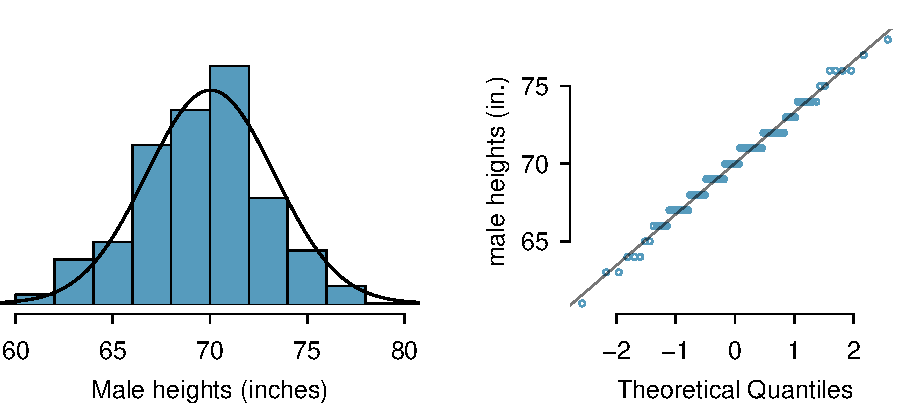
\includegraphics[width=0.9\textwidth]{figures/fcidMHeights/fcidMHeights}
\end{center}

\disc{Why do the points on the normal probability have jumps?}

\end{frame}

%%%%%%%%%%%%%%%%%%%%%%%%%%%%%%%%%%%

%\begin{frame}
%\frametitle{Constructing a normal probability plot}
%
%We construct a normal probability plot for the heights of a sample of 100 men as follows:
%
%\begin{enumerate}
%
%\item Order the observations.
%
%\item Determine the percentile of each observation in the ordered data set.
%
%\item Identify the Z scores corresponding to the each percentile \emph{for a Z distribution}.
%
%\item Create a scatterplot of the observations (vertical) against the Z scores (horizontal)
%
%\end{enumerate}
%
%\pause
%
%\vspace{-5mm}
%
%\begin{center}
%\begin{tabular}{l | c | c | c | c | c}
%Observation $i$	& 1		& 2		& 3		& $\cdots$	& 100 \\
%\hline
%$x_i$			& 61		& 63		& 63		& $\cdots$	& 78 \\
%Percentile	, $i / (n+1)$& 0.99\% 	& 1.98\% 	& 2.97\% 	& $\cdots$	& 99.01\% \\
%$z_i$			& -2.33	& -2.06 	& -1.89	& $\cdots$	& 2.33
%\end{tabular}
%\end{center}
%
%\pause
%
%\disc{How are the Z scores corresponding to each percentile determined?}
%
%\end{frame}
%
%%%%%%%%%%%%%%%%%%%%%%%%%%%%%%%%%%%%

\begin{frame}

\disc{Below is a histogram and normal probability plot for the heights of Duke men's basketball players (from 1990s and 2000s). Do these data appear to follow a normal distribution?}

\begin{center}
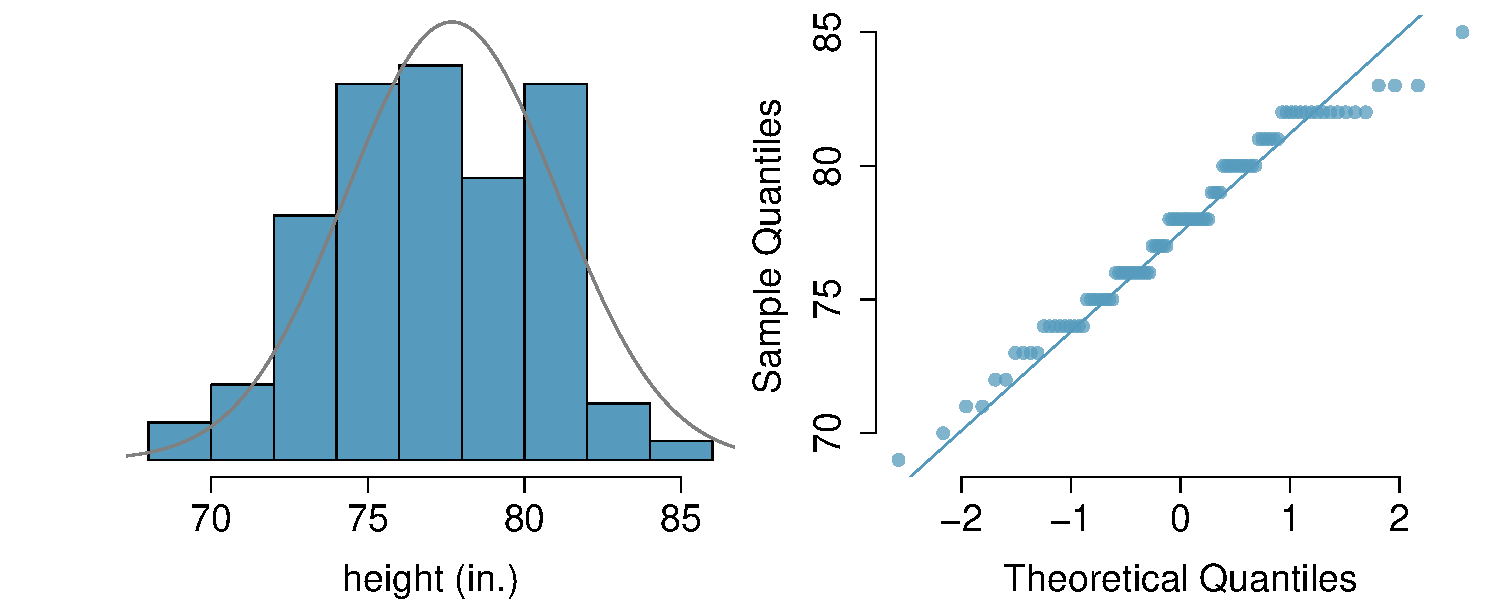
\includegraphics[width=\textwidth]{figures/qq_duke/qq_duke}
\end{center}

\vfill

\ct{Source: GoDuke.com}

\end{frame}

%%%%%%%%%%%%%%%%%%%%%%%%%%%%%%%%%%%

\begin{frame}
\frametitle{Normal probability plot and skewness}

\twocol{0.35}{0.65}{
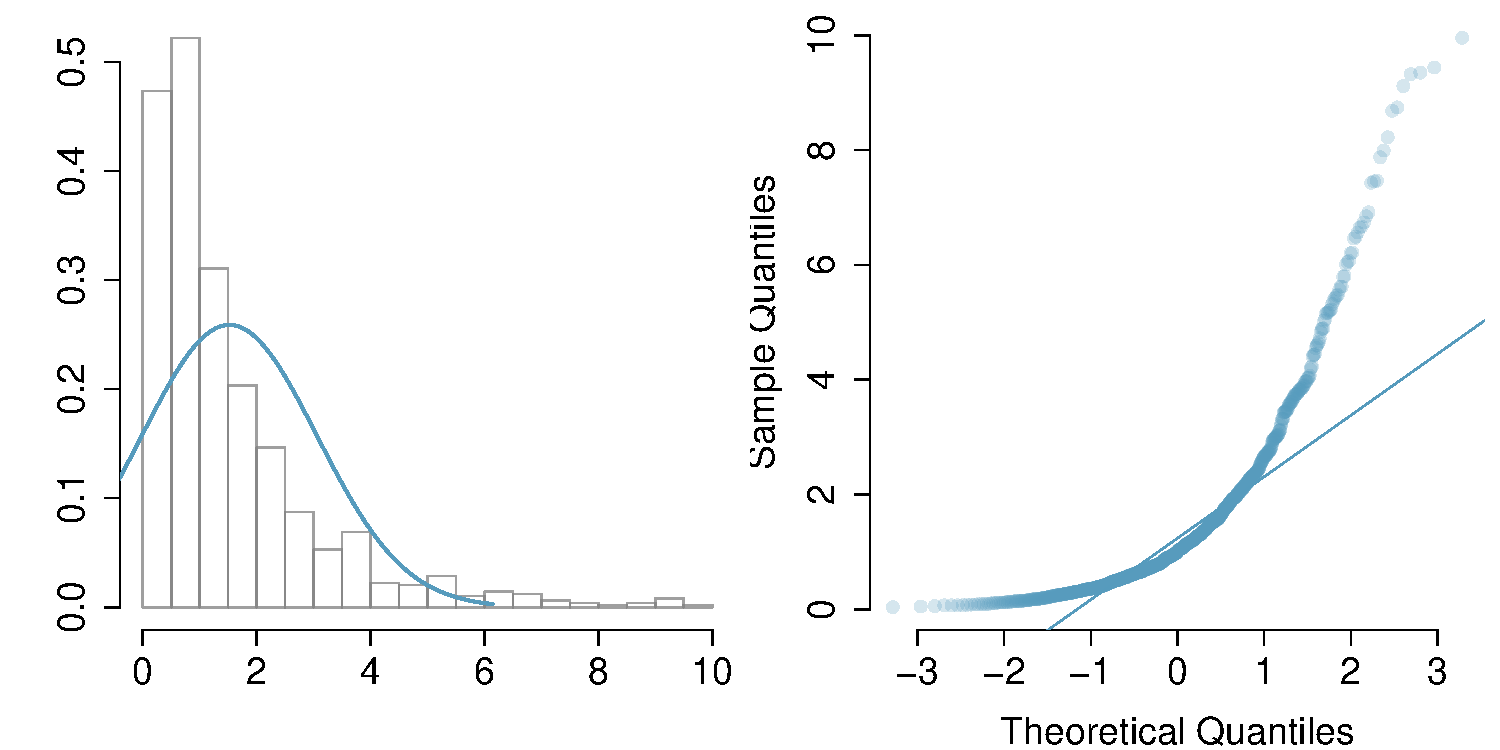
\includegraphics[width=\textwidth]{figures/qqnorm/right_skew} 
}
{
Right Skew - Points bend up and to the left
}

\pause
\twocol{0.35}{0.65}{
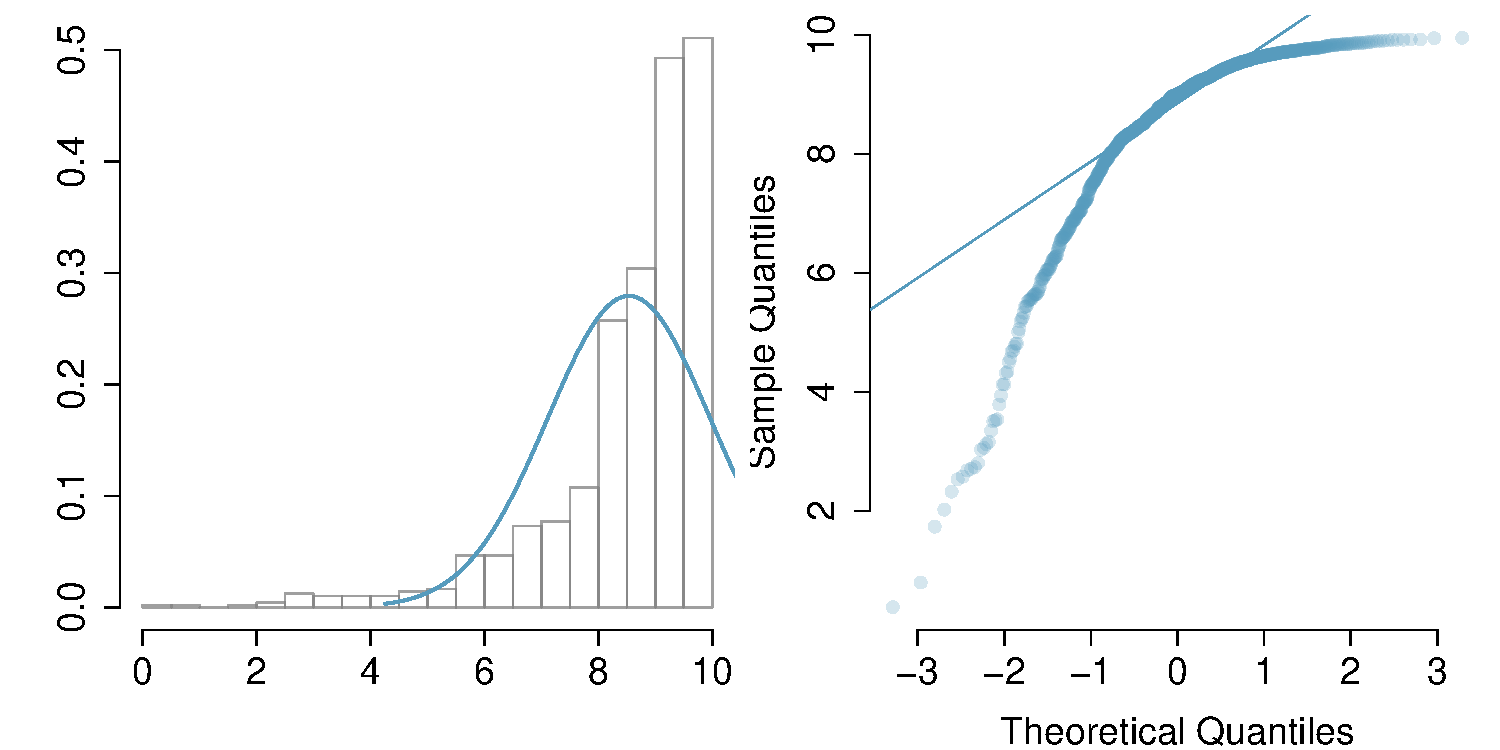
\includegraphics[width=\textwidth]{figures/qqnorm/left_skew} 
}
{
Left Skew - Points bend down and to the right 
}

\pause
\twocol{0.35}{0.65}{
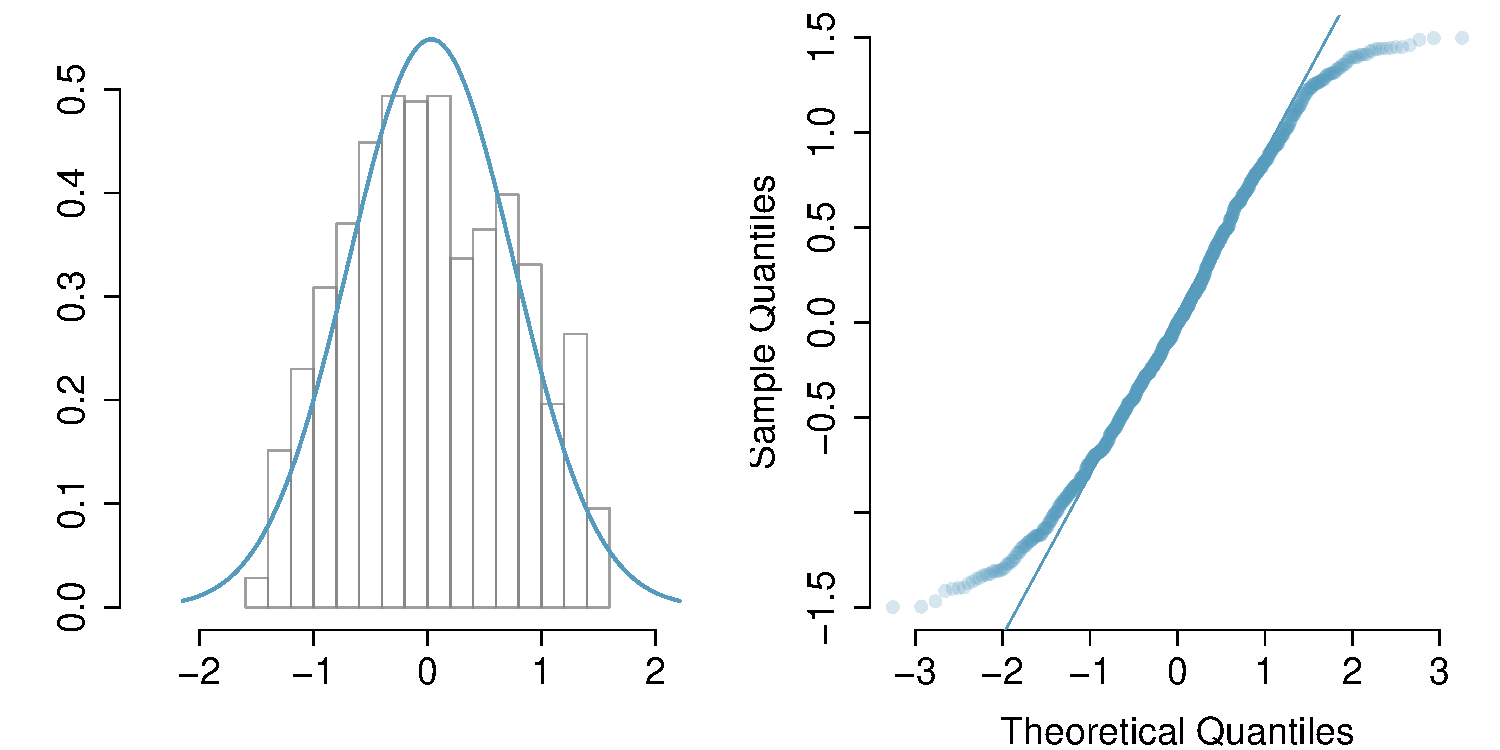
\includegraphics[width=\textwidth]{figures/qqnorm/skinny_tails} 
}
{
Skinny Tails - S shaped-curve indicating shorter than normal tails (narrower, less variable, than expected)
}

\pause
\twocol{0.35}{0.65}{
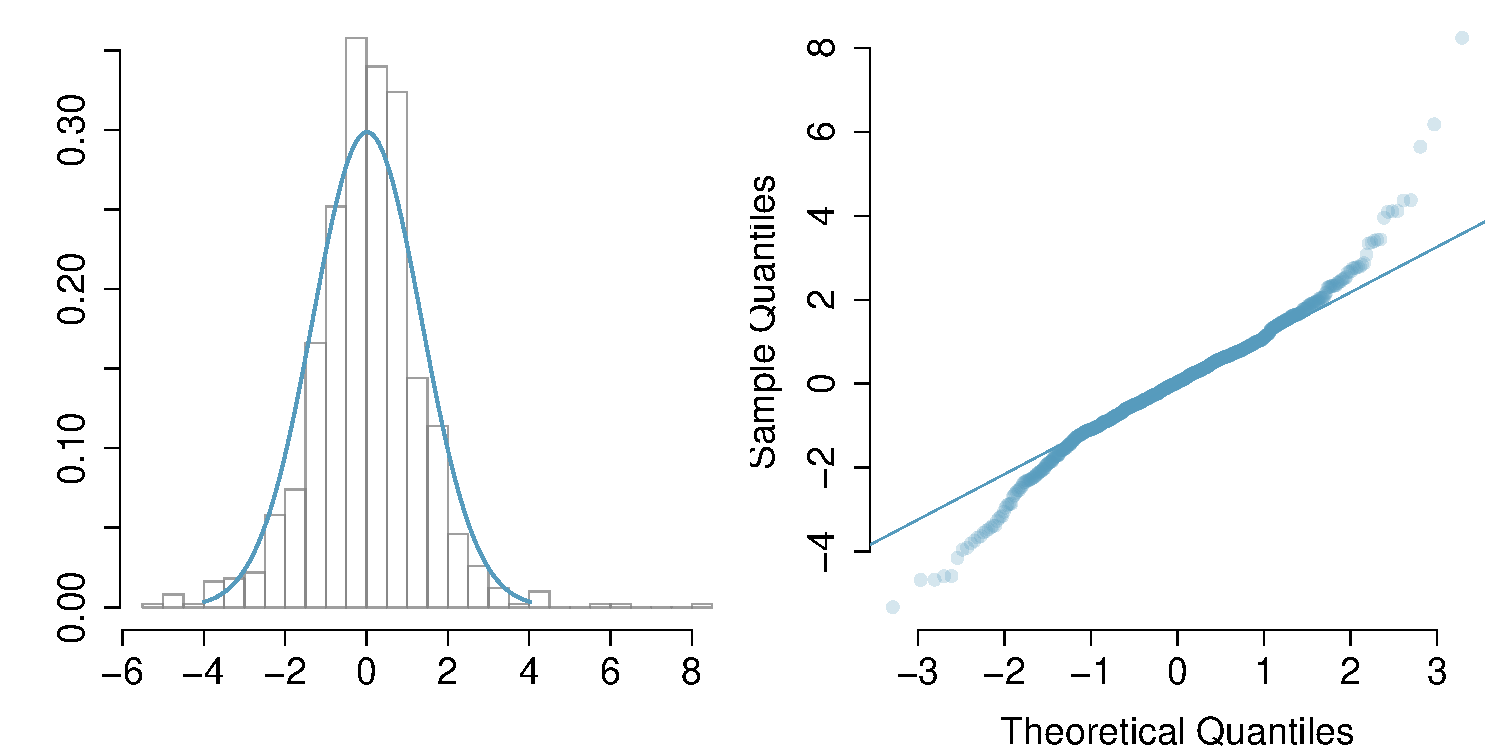
\includegraphics[width=\textwidth]{figures/qqnorm/fat_tails} 
}
{
Fat Tails - Curve starting below the normal line, bends to follow it, and ends above it (wider, more variable, than expected)
}

\end{frame}

%%%%%%%%%%%%%%%%%%%%%%%%%%%%%%%%%%%

\section{Summary}

%%%%%%%%%%%%%%%%%%%%%%%%%%%%%%%%%%%

\begin{frame}
\frametitle{Summary of main ideas - Normal distribution}

\vfill

\begin{enumerate}

\item \nameref{mi1normal}

\item \nameref{mi2normal}

\item \nameref{mi3normal}

\item \nameref{mi4normal}

\item \nameref{mi5normal}

\end{enumerate}

\vfill

\end{frame}

%%%%%%%%%%%%%%%%%%%%%%%%%%%%%%%%%%%

\section{Main ideas - Binomial distribution}

%%%%%%%%%%%%%%%%%%%%%%%%%%%%%%%%%%%%

\subsection{Binomial distribution is used for calculating the probability of exact number of successes for a given number of trials}
\label{mi1binom}

%%%%%%%%%%%%%%%%%%%%%%%%%%%%%%%%%%%%

\begin{frame}
\frametitle{High-speed broadband connection at home in the US}

\begin{center}
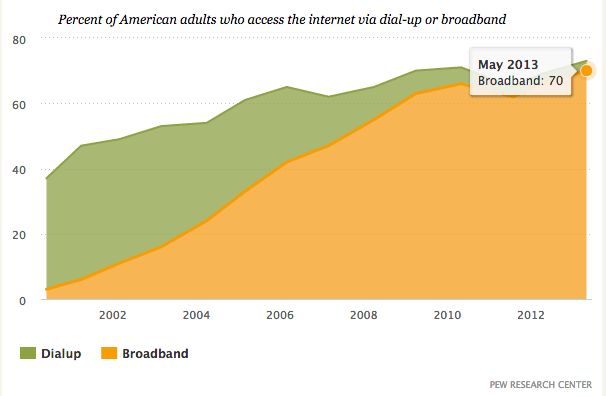
\includegraphics[width=0.6\textwidth]{figures/pew_internet_access}
\end{center}

\pause

\begin{itemize}
\item Each person in the poll be thought of as a \hl{trial}
\pause
\item A person is labeled a \hl{success} if s/he has high-speed broadband connection at home, \hl{failure} if not
\pause
\item Since 70\% have high-speed broadband connection at home, \hl{probability of success} is \hl{p = 0.70}
\end{itemize}

\end{frame}

%%%%%%%%%%%%%%%%%%%%%%%%%%%%%%%%%%%

\begin{frame}
\frametitle{Considering many scenarios}

\disc{Suppose we randomly select three individuals from the US, what is the probability that exactly 1 has high-speed broadband connection at home?}

Let's call these people Anthony (A), Barry (B), Cam (C). Each one of the three
scenarios below will satisfy the condition of ``exactly 1 of them says Yes'': \\
\vspace{0.25cm}
\pause
\begin{changemargin}{+1.5cm}{+0cm}
{\footnotesize
\begin{enumerate}
\item[Scenario 1:] $\slot{0.70}{\text{(A) \red{yes}}} \times \slot{0.30}{\text{(B) no}} \times \slot{0.30}{\text{(C) no}} \approx 0.063$
\pause
\item[Scenario 2:]  $\slot{0.30}{\text{(A) no}} \times \slot{0.70}{\text{(B) \red{yes}}} \times \slot{0.30}{\text{(C) no}} \approx 0.063$
\pause
\item[Scenario 3:]  $\slot{0.30}{\text{(A) no}} \times \slot{0.30}{\text{(B) no}} \times \slot{0.70}{\text{(C) \red{yes}}} \approx 0.063$
\end{enumerate}
}
\end{changemargin}
\pause
The probability of exactly one 1 of 3 people saying Yes is the sum of all of these probabilities.
\[ 0.063 + 0.063 + 0.063 = 3 \times 0.063 = 0.189 \]

\end{frame}


%%%%%%%%%%%%%%%%%%%%%%%%%%%%%%%%%%%

\begin{frame}
\frametitle{Binomial distribution}

The question from the prior slide asked for the probability of given number of successes, \mathhl{k}, in a given number of trials, \mathhl{n}, ($k = 1$ success in $n = 3$ trials), and we calculated this probability as
\[ \#~of~scenarios \times P(single~scenario) \]

\pause

\begin{itemize}

\item $P(single~scenario) = p^k~(1-p)^{(n-k)}$ \\
{\tiny probability of success to the power of number of successes, probability of failure to the power of number of failures}

\pause

\item number of scenarios: ${n \choose k} = \frac{n!}{k! (n - k)!}$

\end{itemize}

\pause
$\:$ \\

The \hl{Binomial distribution} describes the probability of having exactly $k$ successes in $n$ independent trials with probability of success $p$.

\end{frame}

%%%%%%%%%%%%%%%%%%%%%%%%%%%%%%%%%%%

\begin{frame}

\clicker{Which of the following is not a condition that needs to be met for the binomial distribution to be applicable?}

\begin{enumerate}[(a)]
\item the trials must be independent
\item the number of trials, $n$, must be fixed
\item each trial outcome must be classified as a \textit{success} or a \textit{failure}
\item \solnMult{the number of desired successes, $k$, must be greater than the number of trials}
\item the probability of success, $p$, must be the same for each trial
\end{enumerate}

\end{frame}

%%%%%%%%%%%%%%%%%%%%%%%%%%%%%%%%%%%

\begin{frame}[fragile]
\frametitle{Binomial distribution (cont.)}

\[P(k~successes~in~n~trials) = {n \choose k}~p^k~(1-p)^{(n-k)} \] 

\pause

\begin{itemize}

\item You can also use R for the calculation of number of scenarios:
{\footnotesize
\begin{Verbatim}[frame=single, formatcom=\color{blue}]
> choose(5,3)
\end{Verbatim}
}
{\footnotesize
\begin{Verbatim}[frame=single, formatcom=\color{gray}]
[1] 10
\end{Verbatim}
}

\pause

\item And to compute probabilities
{\footnotesize
\begin{Verbatim}[frame=single, formatcom=\color{blue}]
> dbinom(1, size=3, prob=0.7)
\end{Verbatim}
}
{\footnotesize
\begin{Verbatim}[frame=single, formatcom=\color{gray}]
[1] 0.189
\end{Verbatim}
}

\end{itemize}

\end{frame}

%%%%%%%%%%%%%%%%%%%%%%%%%%%%%%%%%%%

\begin{frame}
\frametitle{Properties of the choose function}

\clicker{Which of the following is false? \textit{Hint:} If you're not sure, pick any number for $n$ (choose a low number to make your life easier) and calculate.}

\begin{enumerate}[(a)]
\item There are $n$ ways of getting 1 success in $n$ trials, ${n \choose 1} = n$.
\item There is only 1 way of getting $n$ successes in $n$ trials, ${n \choose n} = 1$.
\item There is only 1 way of getting $n$ failures in $n$ trials, ${n \choose 0} = 1$.
\item \solnMult{There are $n-1$ ways of getting $n-1$ successes in $n$ trials, ${n \choose n-1} = n-1$.}
\end{enumerate}

\end{frame}

%%%%%%%%%%%%%%%%%%%%%%%%%%%%%%%%%%%

\begin{frame}
\frametitle{}

\clicker{According to the results of the Pew poll suggesting that 70\% of Americans have high-speed broadband connection at home, is the probability of exactly 2 out of 15 randomly sampled Americans having such connection at home pretty high or pretty low?}

\begin{enumerate}[(a)]
\item pretty high
\item \solnMult{pretty low}
\end{enumerate}

\end{frame}

%%%%%%%%%%%%%%%%%%%%%%%%%%%%%%%%%%%%

\begin{frame}

\clicker{According to the results of the Pew poll 70\% of Americans have high-speed broadband connection at home, what is the probability that exactly 2 out of 15 randomly sampled Americans have such connection at home?}

\begin{enumerate}[(a)]
\item $0.70^{2} \times 0.30^{13}$

\item ${2 \choose 15} \times 0.70^{2} \times 0.30^{13}$

\item \solnMult{${15 \choose 2} \times 0.70^{2} \times 0.30^{13}$} \soln{\red{\only<2>{$ = \frac{15!}{13! \times 2!} \times  0.70^{2} \times 0.30^{13} = 105 \times  0.70^{2} \times 0.30^{13} = 8.2e-06$}}}

\item ${15 \choose 2} \times 0.70^{13} \times 0.30^2$

\end{enumerate}

\end{frame}

%%%%%%%%%%%%%%%%%%%%%%%%%%%%%%%%%%%%

\subsection{Expected value and standard deviation of the binomial can be calculated using its parameters n and p}
\label{mi2binom}

%%%%%%%%%%%%%%%%%%%%%%%%%%%%%%%%%%%%

\begin{frame}
\frametitle{Expected value and standard deviation of binomial}

\disc{According to the results of the Pew poll suggestion that 70\% of Americans have high-speed broadband connection at home, among a random sample of 100 Americans, how many would you expect to have such connection at home?}

\pause

\begin{itemize}

\item $100 \times 0.70 = 70$
\pause
\begin{itemize}
\item Or more formally, $\mu = np = 100 \times 0.7 = 7$
\end{itemize}

\pause

\item But this doesn't mean in every random sample of 100 Americans exactly 70 will have high-speed broadband connection at home. In some samples there will be fewer of those, and in others more. How much would we expect this value to vary?
\pause
\begin{itemize}
\item $\sigma = \sqrt{np(1-p)} = \sqrt{100 \times 0.70 \times 0.30} \approx  4.58$
\end{itemize}

\end{itemize}

\Note{Mean and standard deviation of a binomial might not always be whole numbers, and that is alright, these values represent what we would expect to see on average.}

\end{frame}


%%%%%%%%%%%%%%%%%%%%%%%%%%%%%%%%%%%

\subsection{Shape of the binomial distribution approaches normal when the S-F rule is met}
\label{mi3binom}

%%%%%%%%%%%%%%%%%%%%%%%%%%%%%%%%%%%%

\begin{frame}
\frametitle{Shape of the binomial distribution}

\vfill

\begin{center}
\webURL{http://bitly.com/dist_calc}
\end{center}
\vfill

\pause

You can use the normal distribution to approximate binomial probabilities when
the sample size is large enough.

\hfill \\

\pause

\hl{S-F rule:} 
The sample size is considered large enough if the expected number of successes and failures are both at least 10
\[ np \ge 10 \qquad \text{ and } \qquad n(1-p) \ge 10 \]

\end{frame}

%%%%%%%%%%%%%%%%%%%%%%%%%%%%%%%%%%%

\begin{frame}
\frametitle{}

\clicker{Below are four pairs of Binomial distribution parameters. Which distribution's shape can be approximated by the normal distribution?}

\begin{enumerate}[(a)]
\item \solnMult{$n = 25, p = 0.45$} \only<2>{\soln{\red{$\rightarrow$ $25 \times 0.45 = 11.25$ and $25 \times 0.55 = 13.75$}}}
\item $n = 100, p = 0.95$ \only<2>{\soln{\darkgray{$\rightarrow$ $100 \times 0.95 = 95$ but $100 \times 0.05 = 5$}}}
\item $n = 150, p = 0.05$ \only<2>{\soln{\darkgray{$\rightarrow$ $150 \times 0.05 = 7.5$}}}
\item $n = 500, p = 0.015$ \only<2>{\soln{\darkgray{$\rightarrow$ $500 \times 0.015 = 7.5$}}}
\end{enumerate}

\end{frame}


%%%%%%%%%%%%%%%%%%%%%%%%%%%%%%%%%%%%

\begin{frame}

\vfill

\app{2.4 Binomial distribution}{See course website for details.}

\vfill

\end{frame}

%%%%%%%%%%%%%%%%%%%%%%%%%%%%%%%%%%%%

 \begin{frame}
 \frametitle{Binomial $\rightarrow$ normal}

 \vfill

 \disc{Why do we care?}

 \vfill

 \end{frame}

%%%%%%%%%%%%%%%%%%%%%%%%%%%%%%%%%%%%

\section{Summary}

%%%%%%%%%%%%%%%%%%%%%%%%%%%%%%%%%%%%

\begin{frame}
\frametitle{Summary of main ideas - Binomial distribution}

\vfill

\begin{enumerate}

\item \nameref{mi1binom}

\item \nameref{mi2binom}

\item \nameref{mi3binom}

\end{enumerate}

\vfill

\end{frame}

%%%%%%%%%%%%%%%%%%%%%%%%%%%%%%%%%%%

\end{document}